%! Author = Johannes Byle
%! Date = 9/8/2021

% Preamble
\documentclass[12pt]{article}
\title{Classical Mechanics Assignment \#2}
\author{Johannes Byle}

% Packages
\usepackage{amsmath}
\usepackage[margin=0.75in]{geometry}
\usepackage{lipsum}
\usepackage{tikz}
\usepackage{pgfplots}
\usepackage{graphicx}
\usepackage{amssymb}
\usepackage{listings}


% Document
\begin{document}
  \maketitle
  \begin{enumerate}
    \item
    \begin{enumerate}
      \item
      Solving the first derivative to find the location of extrema:
      \begin{gather*}
        V(x)=\frac{x^2}{2}-\frac{x_0\sqrt{1+gx^2}}{\sqrt{1+gx_0^2}}\\
        \frac{\delta V(x)}{\delta x}=x\left[1-\frac{gx_0}{\sqrt{gx^2+1}\sqrt{gx_0^2+1}}\right]
      \end{gather*}
      Solving for where $\frac{\delta V(x)}{\delta x}=0$:
      \begin{gather*}
        x=0,\ \pm\frac{\sqrt{g^2 x_0^2-gx_0^2-1}}{\sqrt{g^2 x_0^2+g}}
      \end{gather*}
      Taking the second derivative to evaluate each extremum:
      \begin{gather*}
        \frac{\delta V(x)}{\delta x^2}=\frac{x_0\left(\frac{g^2 x^2}{(gx^2+1)^{3/2}}-\frac{g}{\sqrt{gx^2+1}}\right)}{\sqrt{gx_0^2+1}}+1\\
        \frac{\delta V(0)}{\delta x^2}=1
      \end{gather*}
      This shows us that $x=0$ is a local minimum.
      Not wanting to solve the algebra, simply by looking at the plot of $V(x)$ below we can see that as long as the other extrema exist they will be local minima:\\
      \linebreak
      \begin{tikzpicture}
        \begin{axis}[xmax=3,xmin=-3, samples=100, xlabel=x, ylabel=V]
          \addplot[black] (x,x^2/2-sqrt(1+2*x^2));
        \end{axis}
      \end{tikzpicture}\\
      These minimum will only be real (i.e. exist) if $(g^2 x_0^2-gx_0^2)\geq 1$\\
      \item
      \includegraphics[width=0.75\textwidth]{HW_2_scripts/potential_plot}
      \item The behaviour of the particle will depend on the exact value of $g$ and $x_0$.
      If $g<=\frac{x_0+\sqrt{x_0^2+4}}{2x_0}$, or if $x_0\gg 0$, then the particle will oscillate around $x=0$.
      Otherwise, the particle will oscillate around the other extrema: $\pm\frac{\sqrt{g^2 x_0^2-gx_0^2-1}}{\sqrt{g^2 x_0^2+g}}$.
    \end{enumerate}
    \item\\
    \begin{enumerate}
      \item\\
      \lstinputlisting[language=python, label={lst:bifurcation.py}]{HW_2_scripts/bifurcation.py}
      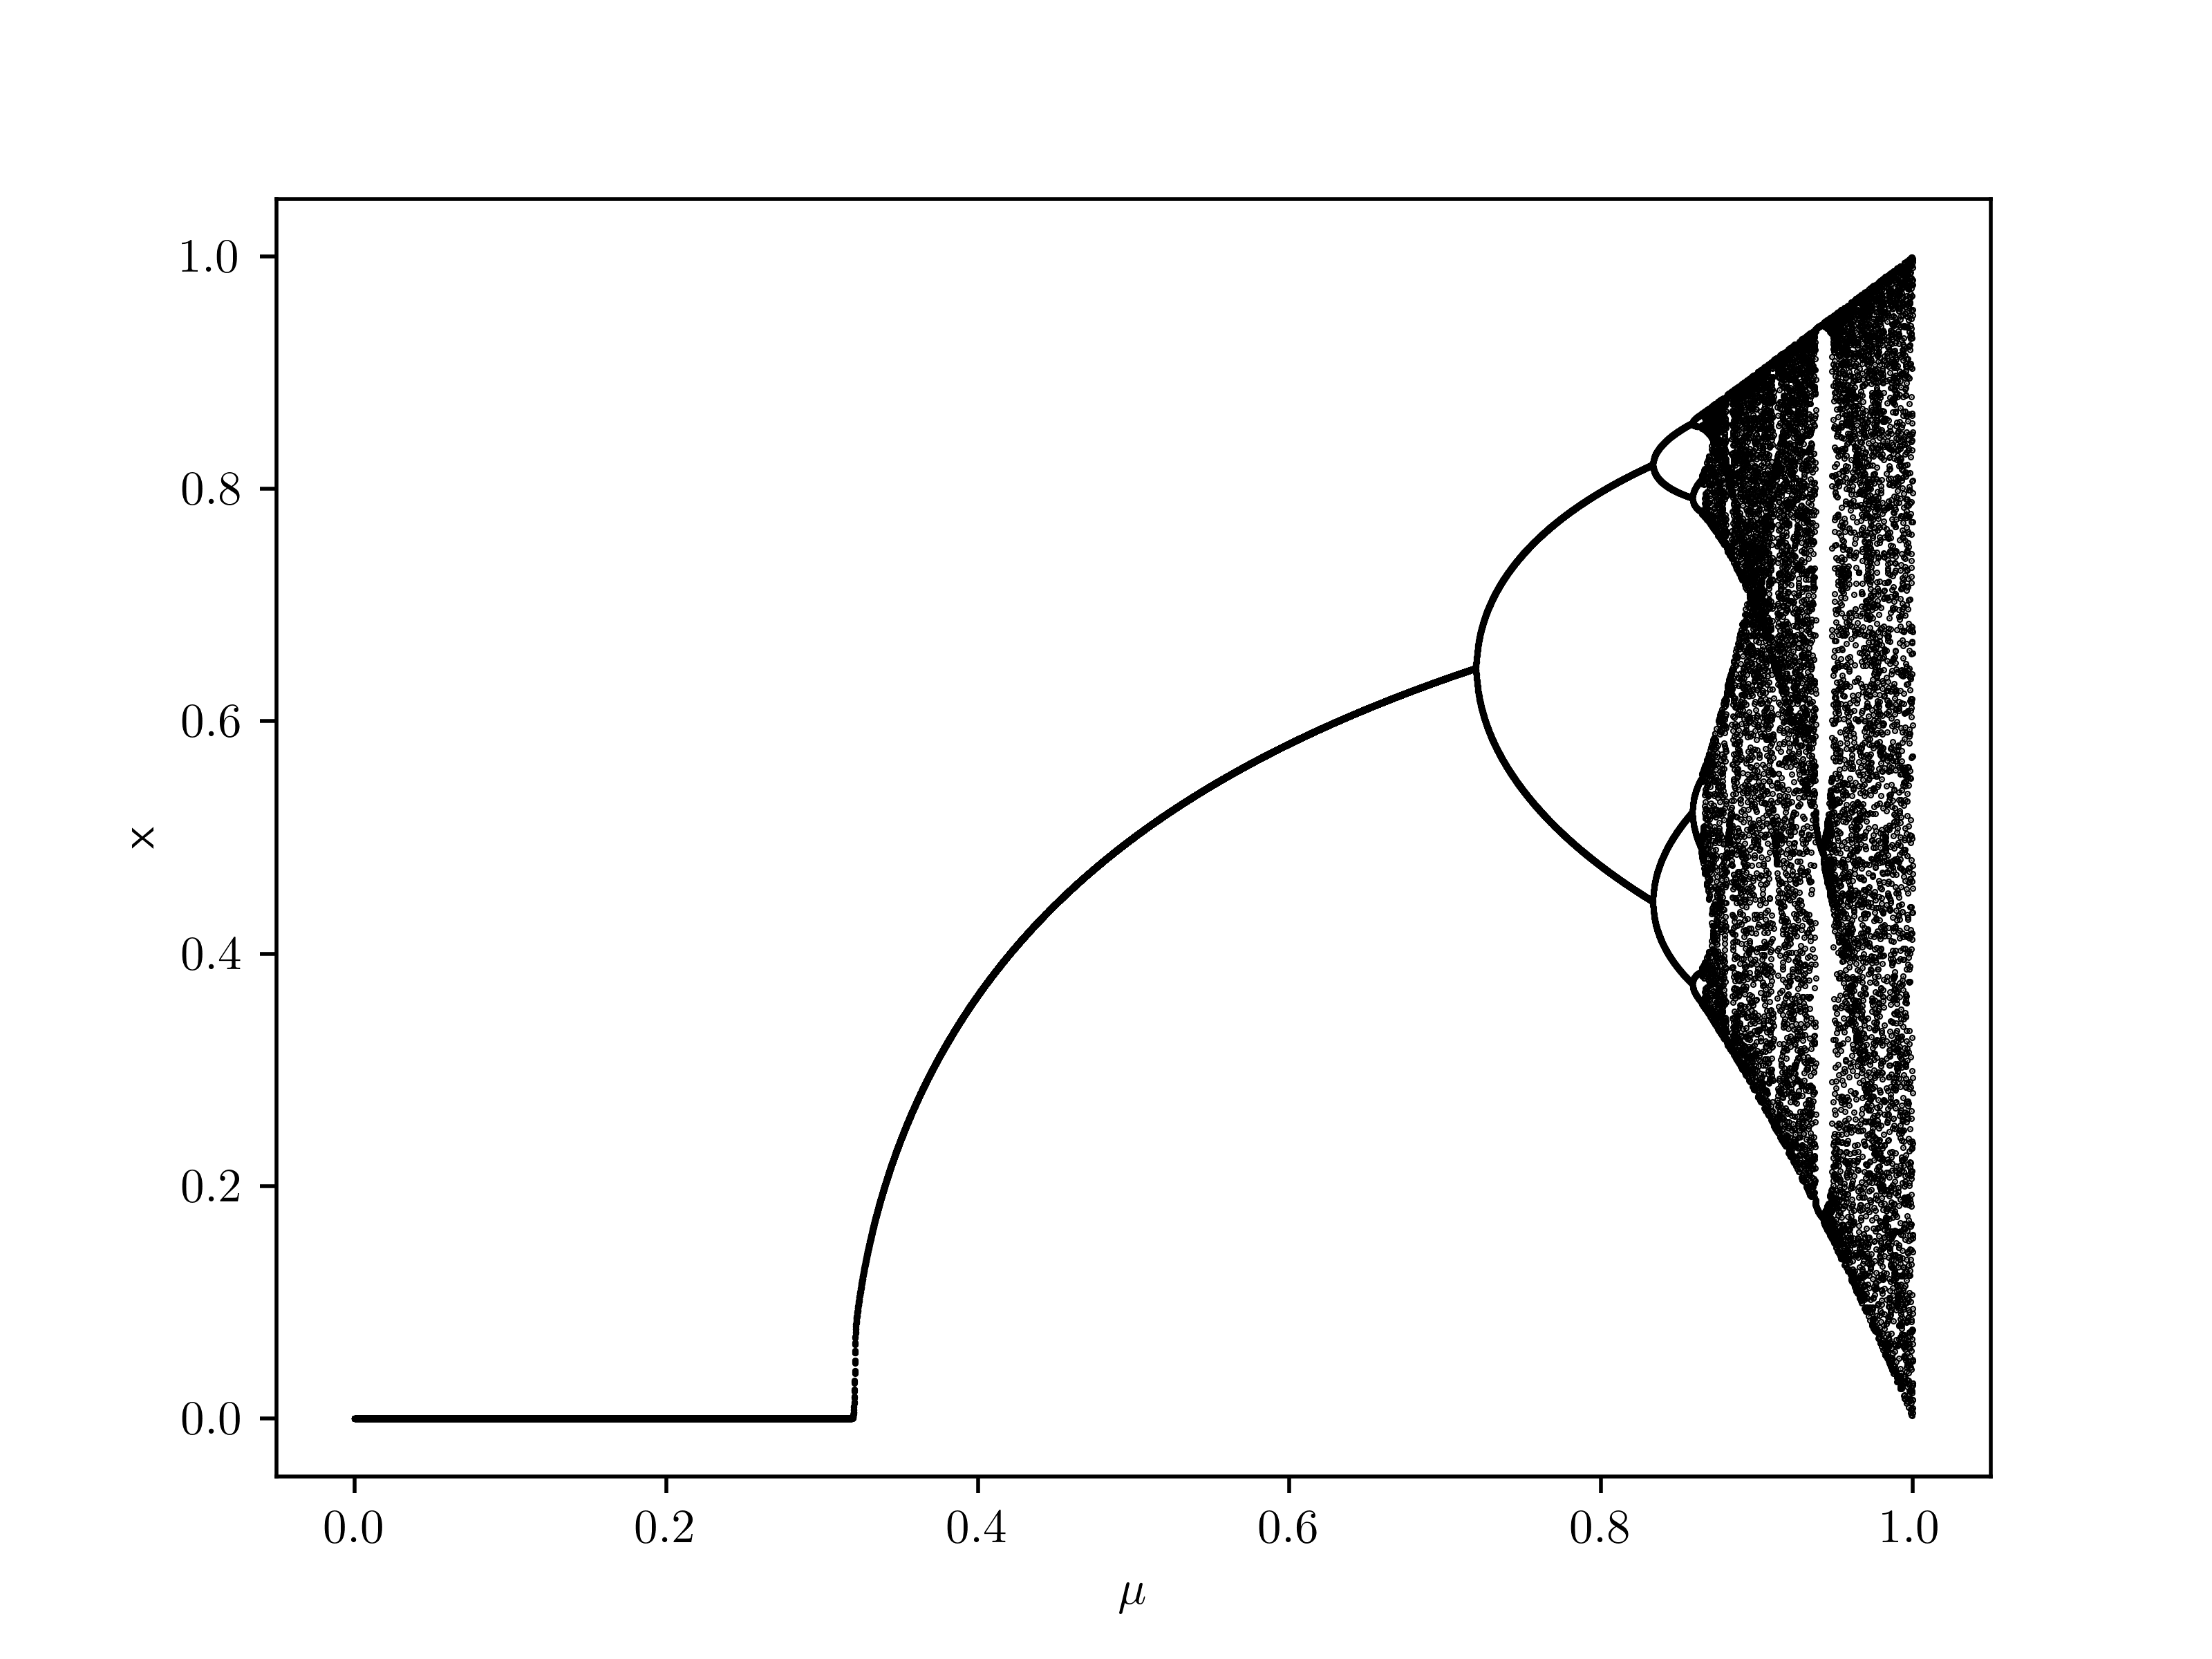
\includegraphics{HW_2_scripts/bifurcation}
      \item
      Fixed points are where $x_{n+1}=x_n=\mu\sin\left(\pi x_n\right)$.
      The first trivial solution is where $x_n=0$ as $\mu\sin\left(\pi\cdot0\right)=0$.
      The second solution is more complicated;
      taking a derivative in terms of $x_n$ and solving for $\mu$:
      \begin{gather*}
        \frac{\delta}{\delta x_n}\left(\mu\sin\left(\pi x_n\right)-x_n\right)=\pi\mu\cos(\pi x)-1\\
        \mu=\frac{\sec(\pi x_n)}{pi}\\
        \mu_0=\frac{1}{\pi}
      \end{gather*}
      \item
      The following plot illustrates the roots of the function $\mu\sin(\pi x)-x=0$ plotted against the derivative of the function $\mu\sin(\pi x)$ evaluated at that root.
      The plot shows that the fixed point is stable until the derivative gets smaller than -1:\\
      \includegraphics{HW_2_scripts/stability}
      \item This is illustrated even more clearly by superimposing the bifurcation diagram onto the plot, and highlighting where the derivative passes -1, as this corresponds to where the fixed point becomes unstable:\\
      \includegraphics{HW_2_scripts/stability_bifurcation}
      \lstinputlisting[language=python, label={lst:stabilty.py}]{HW_2_scripts/stability.py}
    \end{enumerate}
    \item
    Based on the bifurcation diagram below it is clear that it begins to be chaotic at $\alpha=\frac{1}{2}$.
    Thus it is chaotic between $\frac{1}{2}<\alpha\leq1$.
    This can also be seen from the derivative of the function:
    \begin{gather*}
      \frac{d}{dx}\left(2\alpha x-x\right)=2\alpha-1
    \end{gather*}
    Which is zero at $\alpha=\frac{1}{2}$.\\
    \includegraphics{HW_2_scripts/bifurcation_2}
    \item
    \begin{enumerate}
      \item The paper essentially used several methods to find patterns in the evolution of the dynamics of a spring-pendulum system.
      The methods they used included poincare maps at different energies, Lyapunov exponents, Correlation functions, and power spectra.
      The main result of the paper was that at higher energies the system displays greater regions of regularity, as demonstrated by the poincare maps and confirmed by most of the other methods.
      \item The panels went from large negative energies to large positive energies, and showed that going in that direction increased the area of the phase space that showed more regularity.
      This can be seen by the fact that the negative energy panel had very dense areas of chaos, and that the largest reagions of regularity where found in the large energy poincare map of panel (c).
    \end{enumerate}
  \end{enumerate}


\end{document}